\section[Latent Steps]{Latent Steps: Generative Bodily Animations From a Collection of Human Drawings and Physiological Data Interaction}

\label{case_studies:latent_steps}

This case study will be given attention over two segments, a technical primer followed by a user study. The first describes the development process and technical composition of a real-time visualisation system, the next compares this side-by-side with an alternative approach for visualisation, focused on a user perspective. The latter is framed in the following publication effort:

\printpublication{correia_designing_2022}

% Nuno N. Correia, Raul Masu, William Primett, Stephan Jürgens, Jochen
% Feitsch, and Hugo Plácido da Silva. 2022. Designing Interactive Visuals
% for Dance from Body Maps: Machine Learning and Composite Animation
% Approaches. In Designing Interactive Systems Conference (DIS ’22), June
% 13–17, 2022, Virtual Event, Australia. ACM, New York, NY, USA, 13 pages.
% https://doi.org/10.1145/3532106.3533467

% \section{Latent Steps}

\subsection{Introduction}

Latent Steps is an interactive system for dance performance which merges two machine learning models to generate animations using a pre-existing image corpus and physiological data input. The intention is to expose the physical sensations of the user as they revisit a sequence of movements.
The image generation model is trained on a collection of 100 bodily map illustrations (shown in Fig. 1) provided by 10 dancers, who were asked to colour areas of muscular activation and balance during movement. Each drawing correlates to a physical gesture assigned to one of the following semantic descriptors: \textit{Difficult}, \textit{Aesthetic Form}, \textit{Indifferent}, \textit{Open}, and \textit{Closed}. When trained, it’s possible to generate new animations from two or more drawings by predicting the interpolated frames in latent space (Fig. 2). The frames are converted into a UV texture that is projected onto a 3D mesh to highlight particular areas of the body.

The input model, responsible for monitoring the user’s physical activity feeds two control parameters to the Autoencoder model to complete the interaction loop. When a sequence is re-performed, the system will attempt to recognise what pre-defined gesture is being displayed whilst reporting the relative speed of the movement. The result enables users to determine the style of images being generated whilst influencing the time-dynamics of the animation.

\subsection{Background}

\subsubsection{Soma Design Theorey}
The study of the soma considers how the body is perceived from one's proprioceptive senses, emphasising importance on the first-person perspective\cite{hook_embracing_2018}. Somatic practices, such as Contact Improvisation and Feldenkrais are used to develop one’s bodily awareness \cite{tsaknaki_teaching_2019}. In turn, a better understanding with one's own body grants better resources for non-verbal expression, supporting the use of movements and postures to convey emotion. Such practices can improve the participants sense of self, through embodies which can link to improvements in overall well-being \cite{samaritter_aesthetic_2018}. There are a number of methods available to document the bodily sensations manifested as a result of a somatic activity, including the use of biomedical data \cite{hook_soma_2019} as well as visual in the form of bodily map drawings \cite{windlin_soma_2019}. The term somaesthetics was proposed by Richard Shusterman to bind the aesthetic experience (our senses) with the body \cite{hook_somaesthetic_2016}. This concept highlights the importance of bodily movements as a means to experience and exist in the world \cite{shusterman_body_2008}. Somaesthetics has been incorporated into design strategies which aim to orchestrate embodied experiences with sociological materials \cite{tsaknaki_teaching_2019}. In our study, we consider the bodily maps as an aesthetic medium to convey the sensory experience. Instead of mapping kinematic data directly to emotional descriptors, we develop visualisations strategies that can be linked to the user's first-person perception of the interaction.

Several HCI researchers have been exploring the potential of engaging in somatic theories and practices for designing technologies \cite{hook_somaesthetic_2016}. This turn to the body, or the \textit{soma}, as a holistic approach to movements, body, emotions and feelings, is often referred to as a \textit{somatic turn} in HCI \cite{loke_somatic_2018}. It is characterised by a shift to methods of thinking through doing and moving, privileging experiential first person methods \cite{hook_embracing_2018} along with empirical observation and evaluation of users and user experiences.

% One such approach and method that has been of particular interest and motivated our work is soma design (REF. . As suggested in soma design, the materials a designer engages with are not only the digital and physical materials used to build an interactive artifact with, but also the designer’s own (and ultimately) the prospective end-users’ somas [ref].
As movements, experiences and sensory appreciations will be changed, extended and molded through the interactions with a system. There is a variety of soma-based design strategies for engaging with one's soma in interaction design. One such strategy is to repeatedly practice bodily exercises throughout a design process, aiming to sensitize and become more attentive to one's soma. Firstly aiming to improve designers’ somaesthetic awareness, and ultimately design rich experiences with technologies for end users'. The most common bodily practices used in soma design are Feldenkrais or Contact Improvisation (refs), and can be often guided by a somatic connoisseur \cite{schiphorst_self-evidence_2011}, who is experienced in particular bodily practice.

\subsubsection{Body Maps as Somatic Representation}

In soma design methods, before and after doing a session of a somatic practice (e.g. Feldenkrais) or a bodily exercise, it is common to document one's individual experience in a body map, also sometimes referred to as a body sheet \cite{windlin_soma_2019}. In such a body map one can draw and annotate the physical sensations they felt in particular areas of the body, reflecting on one's physiology and bodily experience before and after the session. This can enable one to turn inwards and pay attention to bodily sensations often neglected, including for example pain, discomfort or pleasant sensations. Whilst these drawings are used to aid the participants' verbal description, by themselves, they offer an effective method for documenting an experience in a visual way that moves beyond linguistic and verbal descriptions.

For example, using a colourful pen to draw an experience of pain or a pleasant sensation can be more evocative than describing it with words. Additionally, one can compare their documented felt experiences before and after an exercise, and thus possibly become more aware of how the exercise affected their soma. The body map documentations are also used for sharing and discussing individual experiences in a group of researchers and identify experiential qualities that could drive forward the design work in the group \cite{tennent_soma_2020}. Finally, looking at a body map drawing much later, can remind one of bodily experiences evoked during a particular session of somatic practice done in the past, which could potentially inspire the design of an interactive system that would evoke a similar somatic experience in interaction. This process was carried out in our first case study, detailed in Section \ref{case_studies:soma_chi}.

% As demonstrated in Case Study 1

\subsection{Motivation}

\subsubsection{Limitations of Body Maps}

Our adoption of body maps builds on our long engagement with soma design methods and on our experience of extensively using the body maps in our design processes (in Sections \ref{preliminary_actions:modi_ws1} and \ref{case_studies:soma_chi}, based on our collaborative research actions with the KTH's Interaction Design group, including those teaching soma design \cite{tsaknaki_teaching_2019}. From these experiences, we started identifying a number of limitations of the body maps as a method for facilitating self-reflection and sharing experiences in a group. This work is an attempt to respond to some of the limitations identified, and shows a path towards taking the body maps one step further. Our attempt with the development of the Latent Steps prototype is to suggest a path towards developing tools and mediums that, similar to the body maps, can offer new possibilities for reflecting on one's soma and for documenting such reflections. While, at the same time, keeping the main qualities and properties of the body maps as a useful tool for design processes in HCI, in which somatic practices are core.

The first limitation of the body maps that we identified is that they can only capture an instance, or a static image of a bodily experience. This is due to the existing materiality and actual medium of the maps (a sheet of paper that one can draw on), that enable only a two-dimensional representation of the body. And which also poses constraints when one wants to capture a dynamic experience or sensation felt, such as tension that starts on the neck and moves down along the spine. Moreover, this static representation of the body poses limitations when one wants to represent a movement performed and its impact on the body. Especially since the body is fleshy, alive and active, and the body maps are 2D and static, as mentioned earlier. A third limitation identified has to do with the degree to which they enable and facilitate remembering, or better ``re-feeling'' a documented experience, when returning to a body maps later in time (e.g. after a few weeks). Through our experience with using the body maps we noted that even though they provide a means of documentation that can be kept, stored, and retrieved later, it is often challenging to remember the exact experience, sensation or impact that an exercise has left on the body.

So we begin questing: How can we expand the possibilities of the existing body maps and create a more ``alive'' type of body map, in line with the aliveness of our moving and fleshy somas? At the same time we were interested in exploring possibilities of allowing a person to make their own data set of articulated bodily experiences over time, which could probably provide an added value to the existing use of the body maps: To enable reflections on the living and changing body over time, including movements and micro movements performed.

% \begin{figure}[ht]
%     \centering
%     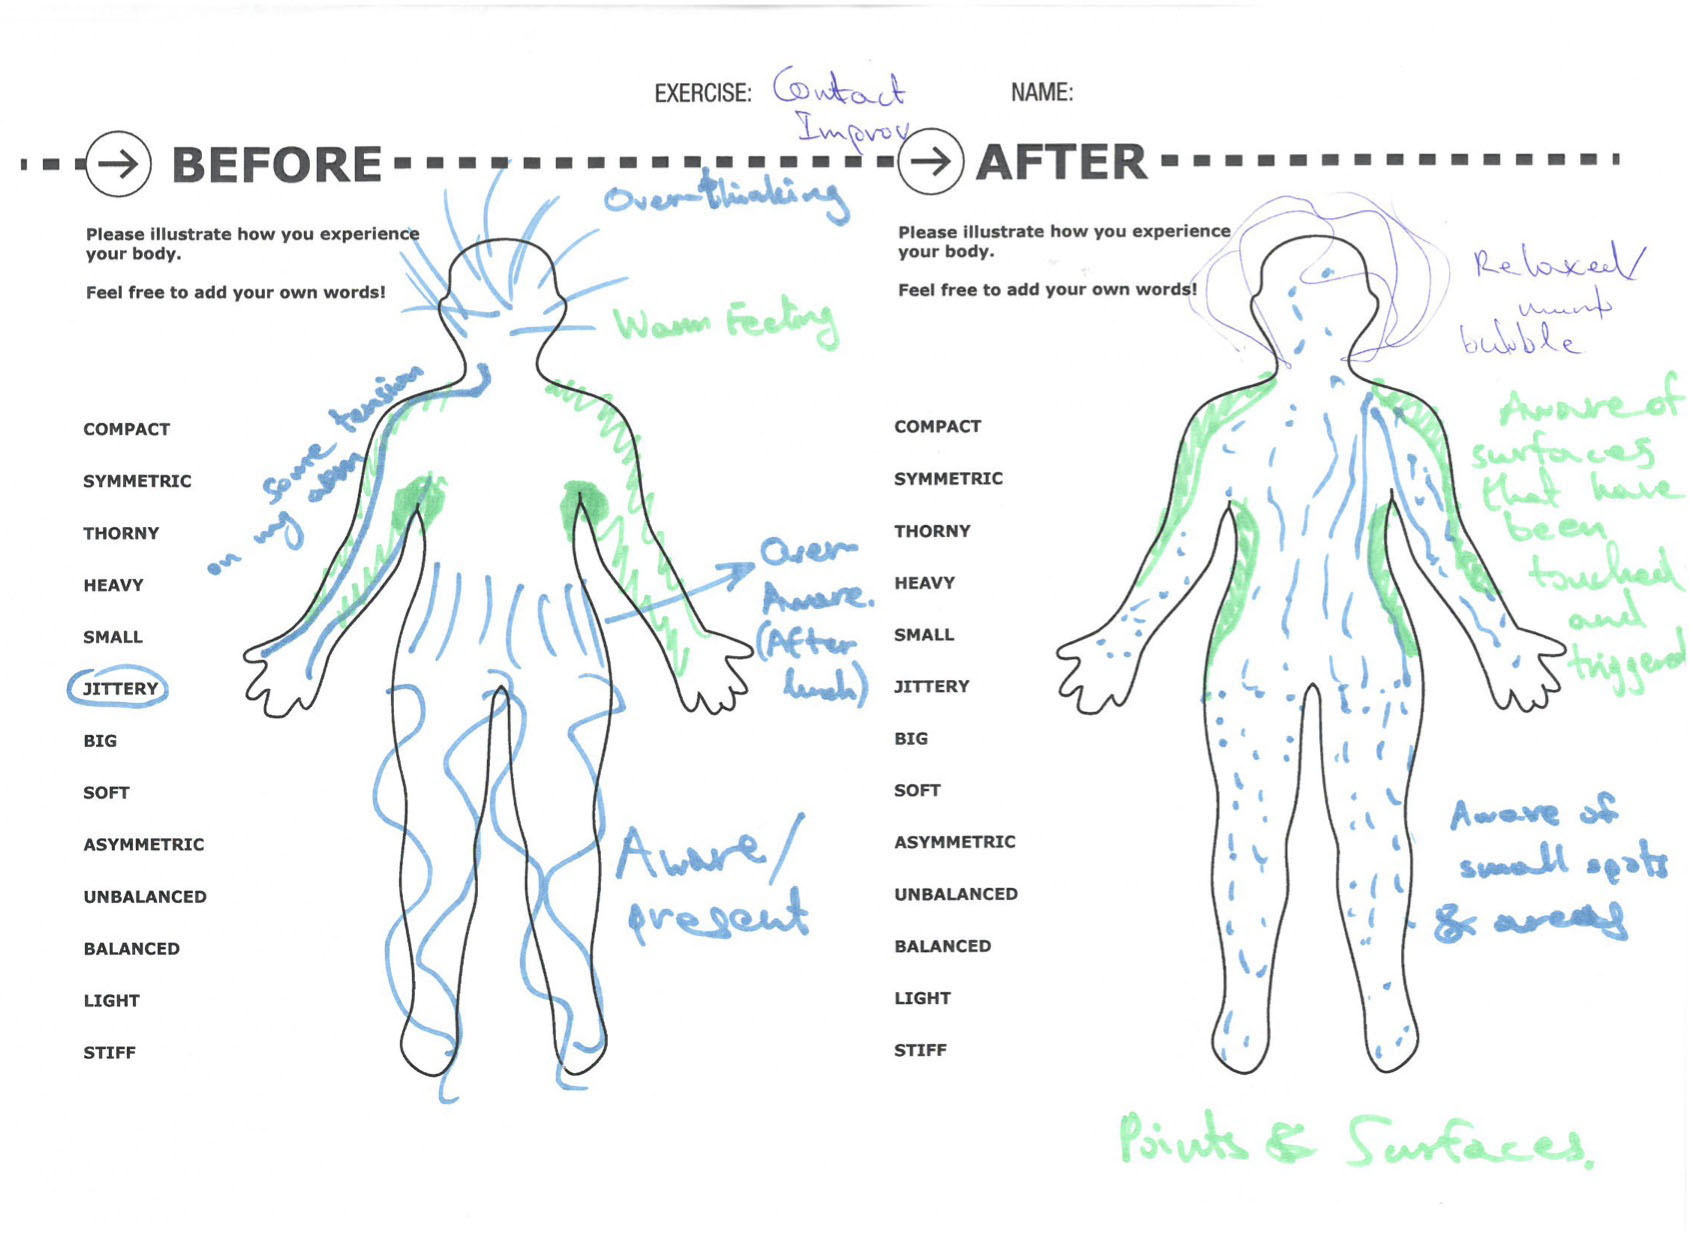
\includegraphics[width=0.75\textwidth]{Chapters/Figures/modi_dis/kth_body_maps.jpg}
%     \caption{Example of a body map used in the workshop to document bodily experiences before and after each workshop activity.}
%     \label{fig:draw_samples}
% \end{figure}

\begin{figure}[ht]
    \centering
    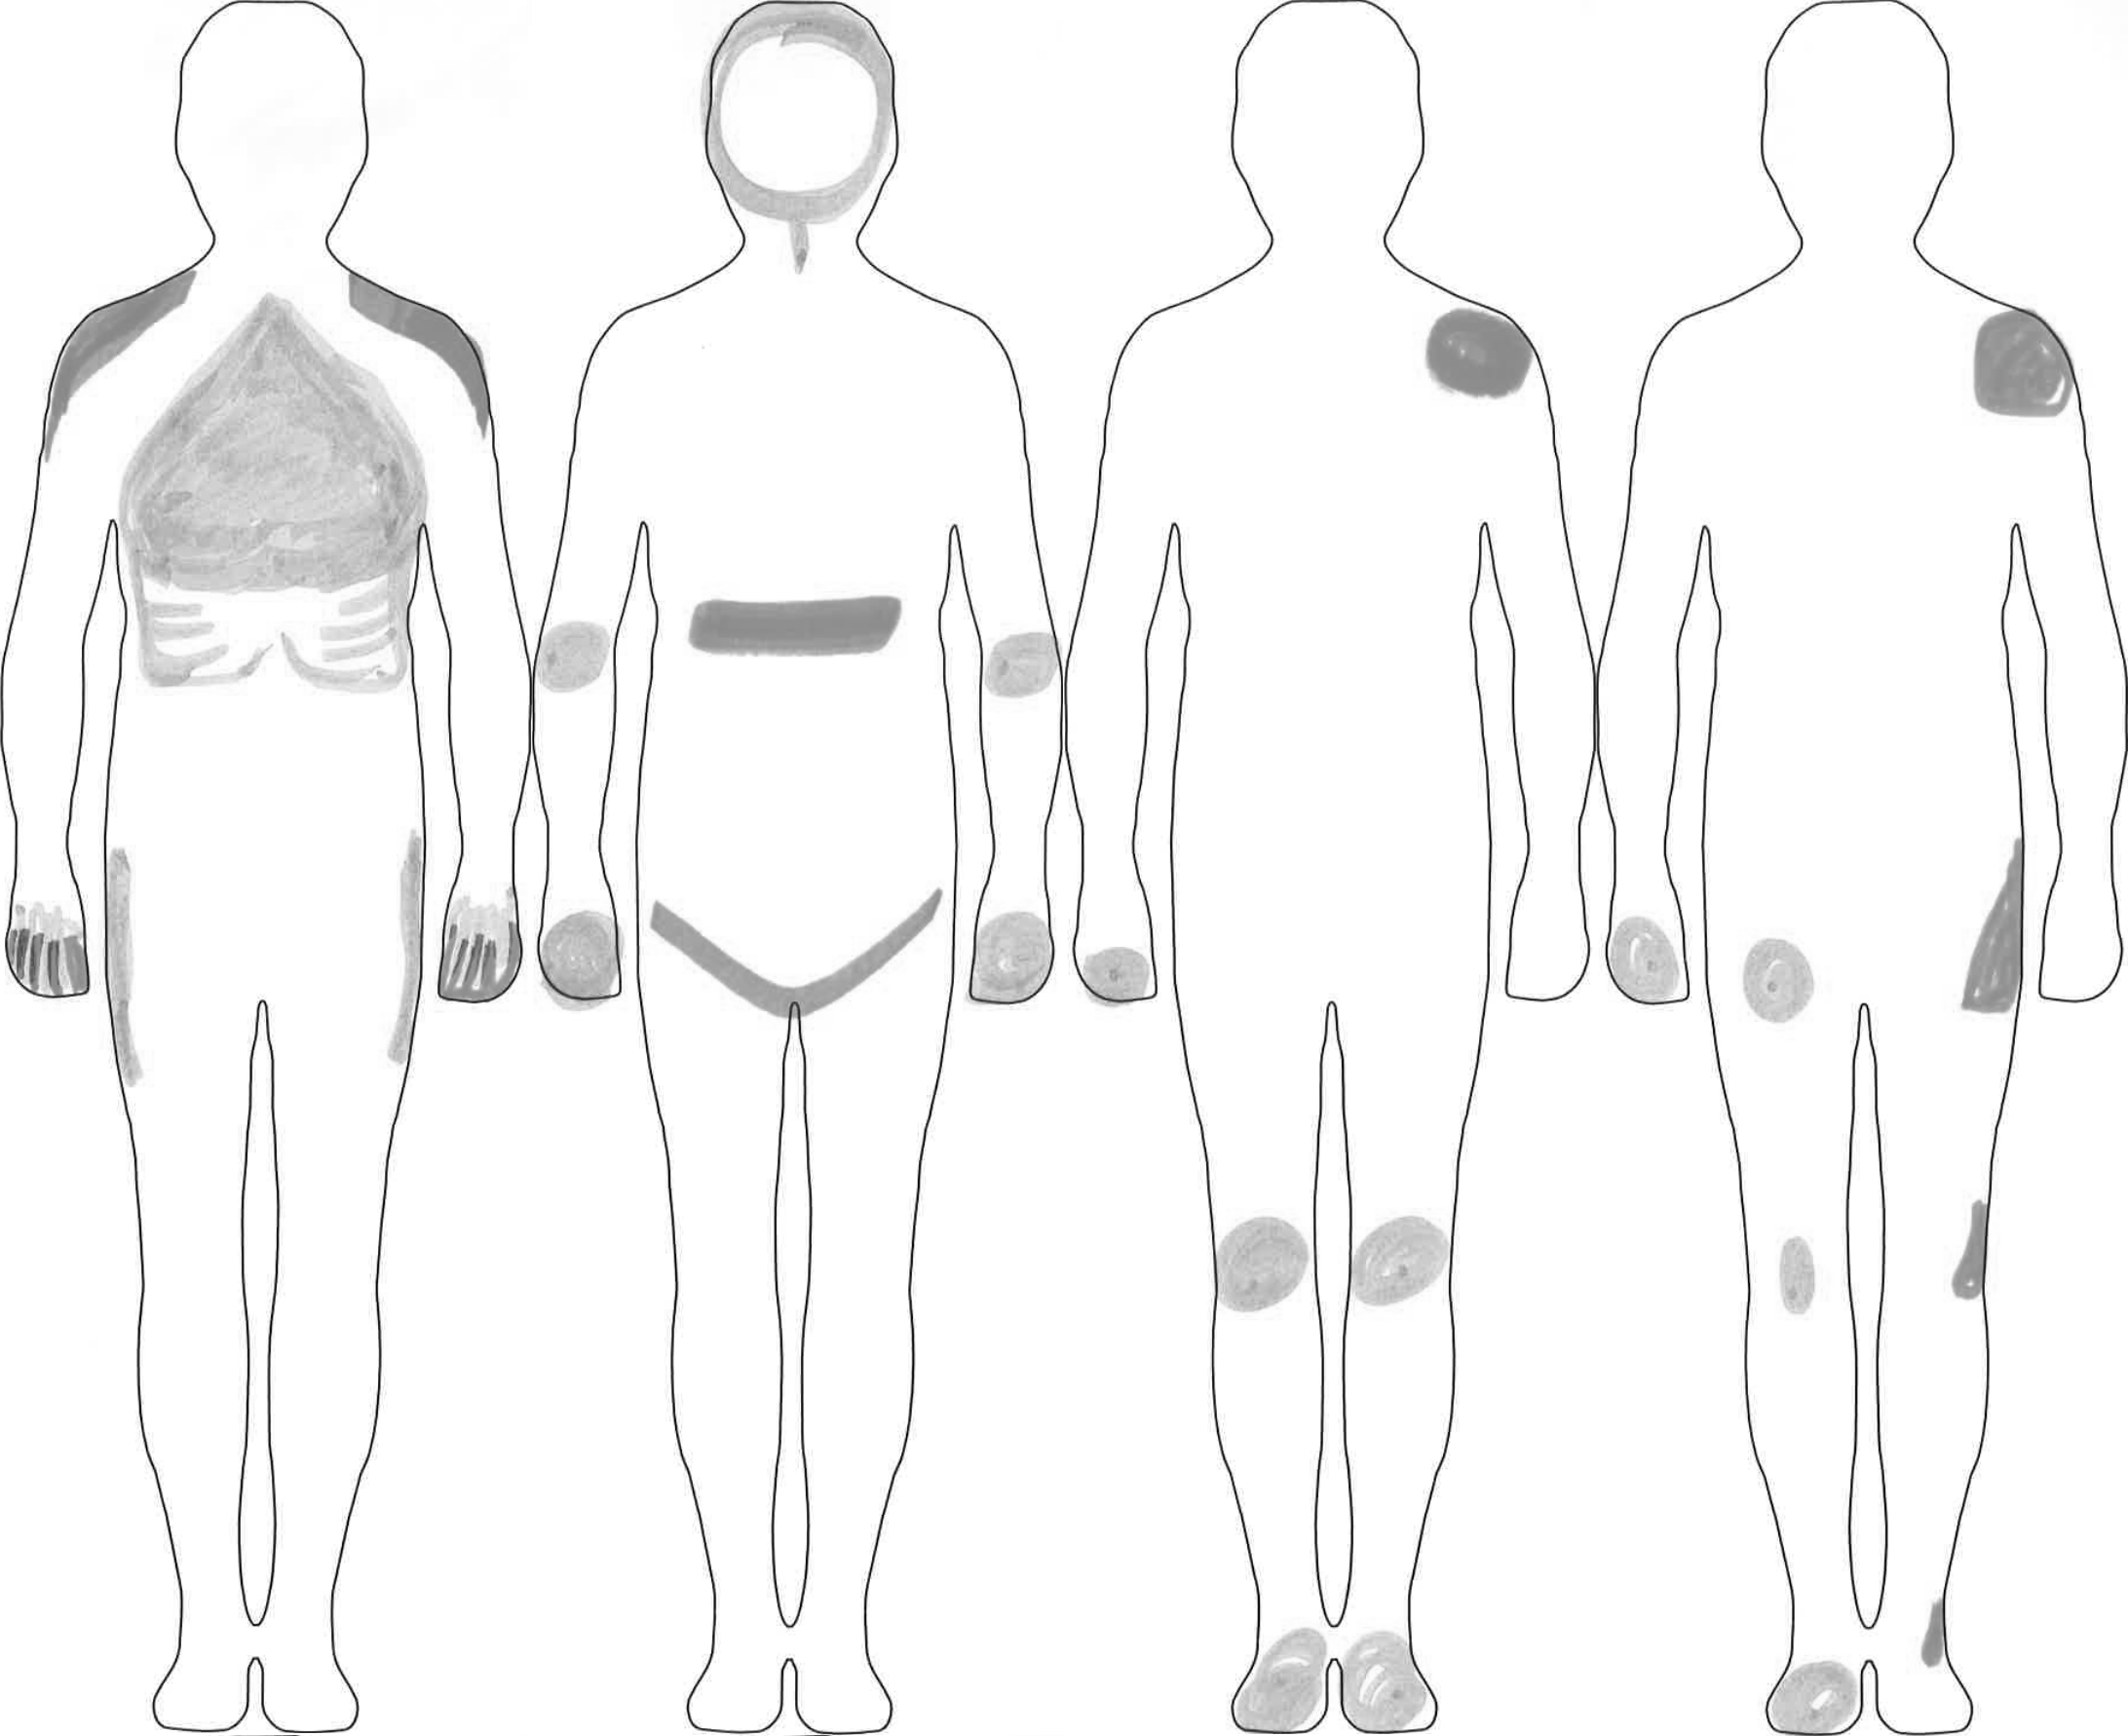
\includegraphics[width=0.70\textwidth]{Chapters/Figures/modi_dis/drawing_samples2.png}
    \caption{Four Examples of Body Sheets used in Latent Steps.}
    \label{fig:draw_samples}
\end{figure}

\subsubsection{Interactional Approaches to Designing with Bodily Data}

We can use Affective Computing as an example. Affective Computing is representational, as in it describes certain aspects emotions in numerical terms, derived from measurements in the body. Affective Interaction systems, on the other hand, create representations that do not attempt to be true and objective, but rather depend on the users engaging with them and interpreting them. We ascribe this to an interactional approach. As \citeauthor{hook_affective_2009} put it, \textit{“An interactional perspective on design will not aim to detect a singular account of the “right” or “true” emotion of the user and tell them about it as in a prototypical affective computing application, but rather make emotional experiences available for reflection \cite{hook_affective_2009}. Such a system creates a representation that incorporates people’s everyday experiences that they can reflect on. Users’ own, richer interpretation guarantees that it will be a more “true” account of what they are experiencing.”}

Latent Steps, presented in this section, is more on the interactional side. It creates representations of bodily states and postures but relies on end-user training and configuration of the system and ultimately on end-user personal interpretation. Its aim is not to classify and predict objectively a human posture (we can find in literature many other systems that attempt to predict if the user is sitting or standing or going on a bike based on wearable acceleromters \cite{slim_survey_2019}), but rather to provide cues and tips for personal reflection to emerge, interactively with the system.

\subsubsection{Interactional Approaches to Machine Learning}

The same distinction between representational and interactional can be made for machine learning applications, as it is explained by \citeauthor{gillies_understanding_2019} \cite{gillies_understanding_2019} \cite{bishop_non-representational_2014}. We aim to apply user-centered, interactive machine learning to body maps, which accepts users are the domain experts in their own bodies. They can create a particular language of interaction, adapting a given model, providing training data themselves. In soma design theory, first-person interpretation of bodily data is crucial here. Rather than relying on a population of users and attempting at classifying user data into fixed categories (a representational system), the goal is to design a system that is intended for iterative interactions that end up in the users gaining knowledge about themselves.

\subsubsection{Image Generation with Convolutional Autoencoders}

Convolutional Autoencoders (CAEs) have been used to reduce the dimensionality of images, such as those in the MNIST dataset \cite{wang_auto-encoder_2016}. Between the decoder and encoder functions of the trained machine learning model is the bottleneck layer, composed of compressed representations of the input data \cite{zhang_better_nodate}. In the case that the model has been trained on a corpus of images, we are able to reconstruct the visual data from the compressed vector. From this stage, we are also able to use vector arithmetic to generate new variations of the images that are not contained in the original dataset.

Given the bottlneck layer requires lower dimentionality data to generate a full scale output, it's more feasible to construct interactive mappings with low dimensional inputs. In our system, we interface physiological sensor data with a Convolutional Autoencoder (CAE) for image generation.

\subsection{Technical Composition}

\subsubsection{System Architecture}

The aim of the system is to continuously generate bodily map images that correspond to postural data, which is determined by a set of embodied sensors. The frames are then saved as a means for recording the first-person experience. The frames are then concatenated to produce a video steam that can be used for self-reflection after the activity takes place.

The system utilises two machine learning models across two processes. The training process takes data from a corpus of images and sensor values as input for each model respectively. The learnt model enables continuous mappings to be generated based on these inputs. The interaction process relies on the previously trained models and takes IMU data in real-time to generate reconstructed images. Our workflow is illustrated in Figure \ref{fig:system_overview}.

\begin{figure}[ht]
    \centering
    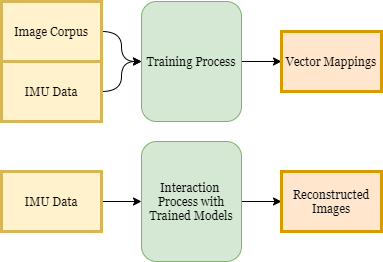
\includegraphics[width=\textwidth]{Chapters/Figures/modi_dis/Latent-Steps-Architecture.png}
    \caption{System Overview.}
    \label{fig:system_overview}
\end{figure}

\subsection{Overview of Hardware and Software}

We are placing five BITalino R-IoT devices\footnote{BITalino R-IoT: \url{https://bitalino.com/en/r-iot-kit}} on the body of the user, each device includes an Inertial Measurement Unit (IMU) to measure the relative orientation of the user’s limbs. We chose to place sensors in the following areas to represent the postural features of the user: upper left and right arm, abdomen, and the up left and right knee. We proposed this solution as a low-dimensional estimator of posture sufficient to differentiate and interpolate between a small set of postures.

% \begin{figure}[ht]
%     \centering
%     % \includegraphics[width=\textwidth]{img/image-placeholder-350x350.png}
%     \caption{IMU Sensor Placement.}
%     \label{fig:placement}
% \end{figure}

The absolute orientation of the sensors are computed within the firmware of the sensor module using the formulas provided in the BITalino R-IoT firmware\footnote{BITalino R-IoT firmware: \url{https://github.com/BITalinoWorld/firmware-bitalino-riot}}. The firmware implements Sebastian Madwick’s algorithm for orientation filtering \cite{madgwick_ecient_nodate}.

The first model, which is trained in the image corpus is programmed using the TensorFlow library \cite{abadi_tensorflow_2016} in Python and the second model, responsible for processing sensor data is implemented in an OpenFrameworks\footnote{openFramworks: \url{https://openframeworks.cc/}.} application using the RapidLib C++ library\footnote{ofxRapidLib: \url{https://github.com/mzed/ofxRapidLib/}} for interactive machine learning.

\subsubsection{Latent Space Conditioning}



\subsection{Training Process}
\label{training_process}

Using the first model, we train a Convolutional Autoencoder (CAE) to interpret the visual features of the image dataset. The model used in our system encodes each image into 32 float vector representations. These vectors are then used as labels when training the regression model. This second model then takes the static postures recorded with IMU  data as an input and produces vector mappings according to the labels (see Figure \ref{fig:training_fig}). The two models are described in further detail in the respective subsections below.

\begin{figure}[ht]
    \centering
    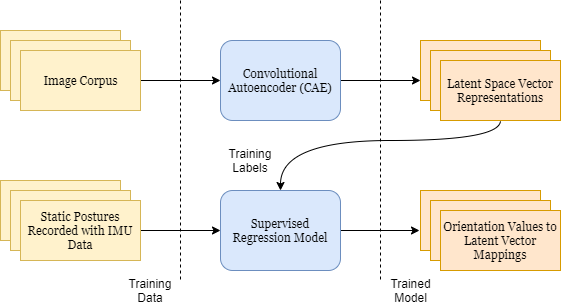
\includegraphics[width=\textwidth]{Chapters/Figures/modi_dis/training_process.png}
    \caption{Training process for the Regression and Autoencoder model.}
    \label{fig:training_fig}
\end{figure}

\subsection{Convolutional Autoencoder Model}

The Convolutional Autoencoder (CAE) is an unsupervised machine learning model, where by the training data is not labelled, independent from any categorical descriptor. The training process initialises with an encoder function that compresses the images into vector representations of 32 floats, corresponding to their relative position in the latent dimension. This compressed representation of the image is assigned according to the visual features interpreted by the model, commonly referred to as latent space. As a result, drawings that are more visually related can be described as closer together, where as dissimilar inputs are located further apart in the latent space.

\[ f:i_n\xrightarrow{}v^n = \{V_0, V_1,... ,V_{32}\} \]

We can state this formula where \textit{i} is the complete 256 x 512 pixel representation of a given image with ID of \textit{n} and \textit{v} is the latent vector (32 float values) produced by the autoencoder.

The decoder function takes the latent vector as an input and reconstructs a new image, incorporating visual features from the training dataset. The decoder can produce the close-to-identical image to that of the original dataset, by feeding the same vector calculated by the encoder. In addition to this, we can also generate continuous interpolations between the drawings when applying vector arithmetic, resulting in a new image that the model has not been explicitly trained with. To evaluate the capabilities of our model, we will apply similarity measurements comparing the reconstructed output to the training data (described in further in section \ref{data_analysis}).

\subsection{Supervised Regression Model and Sensor Input}\label{sensor_input}

We are using {5} Inertial Measurement Units (IMUs) to measure the relative orientation of the user’s limbs. We chose to place sensors in the following areas to represent the postural features of the user: {upper left and right arm, abdomen, and the up left and right knee}. From each IMU, we calculate 4 Quaternion angles to depict the  absolute orientation in 3-dimensional space. Our main motivation for using Quaternions is that the output operate on sine and cosine functions, meaning the values do not skip from minimum to maximum (or visa versa) when reaching the angular thresholds, making this encoding suitable for interpolating between gestures.
% From here, the values are transmitted to the host computer wirelessly using the Open Sound Control (OSC) protocol at a constant 100ms interval.

For every generated image that we want to associate with a particular posture, we store the associated latent vector, used as a continuous numerical label when training the model. For each label, we record 5 seconds of the posture being executed, resulting in approximately 50 examples of each pose. In our experiment, each user will train 4 gestures with a latent vector. When the model is trained, the model will reproduce the latent vector as labelled when a pose is repeated, or if a new posture is provided, the regression function will interpolate between the 4 vectors accordingly to generate a new visual output.

\subsection{Interaction Process}

The interaction loop is completed when we feed the output of the regression model directly to the bottleneck layer of the CAE. Where \textit{p} is the posture represented by orientational values from the sensors and \textit{v} is the latent vector representation of a particular image \textit{i} from the training dataset, we can bridge data from the two models with the following formula:

% \begin{equation}
\[ f:p_n\xrightarrow{}v^n \xrightarrow{}i_n \]
% \end{equation}
% TODO:Label and ref

\subsection{User Feedback \& Discussion}

For our initial evaluation, we will give attention to the remarks provided as part of the user-centred design workshops that proceeded the case study presented in the following Section \ref{case_studies:modi_dis}. To maintain a relevant discussion for this segment, we pick out only the specific points directed towards the Latent Steps system.

\subsubsection{Embracing Data Collection as Aesthetic Experience}

While it was not an intended outcome of the system, the therapeutic quality of the drawing process can surely be acknowledged as complimentary to the holistic user experience. This method of data collection is inherently disruptive, halting the primary activity, and prompting users to pay attention to the internal bodily experiences occurring in that moment. This exercise aligned with some of the core principles of Feldenkrais and even aspects of traditional forms of art therapy. When applying this data into Latent Steps visualisation system, we demonstrate the case for user empowerment through technical transparency, advocating for human-centred workflows. Participants are exposed to the data collection and training processes as they reenact these steps as a prerequisite before they can interact with the predictive visualisation model.

\begin{center}
\begin{tabular}{ p{13cm}}
\textit{But it's also a tool that we somehow coded, like participating in the process of coding, because technology always holds the information of the one who coded it. So it's like biased towards our own body, it's not like something coming from outside, but it's coming from our own somatic awareness. So that's going into ourselves, but also into our own perception.}
\end{tabular}
\end{center}

\begin{center}
\begin{tabular}{ p{13cm}}
\textit{because the way I understand the system, he took our own notations from Tallin, he combined it with the sensor information and then inside his prototype, if we are repeating movements, it provokes the imagery according to our own notation. So there is this kind of introspective way of notating our own movement, which is provoked by this kind of so-called "objective" measurement.}
\end{tabular}
\end{center}

\subsubsection{Issues of Anthropomorphic Representations and Designing for Pluralism}

\begin{center}
\begin{tabular}{ p{13cm}}
\textit{Because I think he used the mapping on the human body, so in this sense I... that's why  think it comes from, or it was already like this anthropomorphic thing was very dominant already from the exercise there. And I agree, for me it was a very... the aesthetic of this output and the human form, for me it was very limiting while using it.}
\end{tabular}
\end{center}

\begin{center}
\begin{tabular}{ p{13cm}}
\textit{And the limitations are indeed in this kind of visualisation of the information in the terms that there are patterns of visualising and immediately when he started with this other (?) that looked too much like a male body, we asked him to delete somehow the male body and then we came up with the aspect of the more abstract figure that you see only the body parts that are shaped, instead of seeing the whole body. And then, I think it was more coming from me, but we all stayed with it, I think it was more appealing in general even. And because the abstraction of it started to open more room for} imagination.
\end{tabular}
\end{center}

We were made highly aware of the issues that arose from the anthropomorphic model used as a geometric outline, especially as depicted the 3D render, that came across as fundamentally unappealing to the user group. The stock avatar that was used originally embodied highly male-orientated attributes which did not resonate strongly with the user's perception of their own body. This sentiment justifies the inclination for a more abstract figure that were more visually consistent with the original body map data.

Here, it is interesting to point out that users coming from marginalised groups, commonly feeling less represented by mainstream avatar representations, express their appreciation towards more abstract forms of the body \cite{niehaus_making_2021}. Correspondingly, ``monster'' body maps and the flexibility from a normative human figure has shown to offer a dynamic understanding of the body \cite{hook_soma_2019}

\subsection{Future Work}

\subsubsection{Separating Layers of Interaction, Representation through Pre-Rendered Material}

The alignment of sensory readings to specific bodily areas came with a few issues, as described above. Favouring abstract representations not only for sensation, but for the presentation of the human from, the artists preferred using the sensory input to interact with the sonic layers while visuals would be project separately. This new configuration was used to develop two public presentations, the first of which which we obtained audience feedback regarding the the audio and visual material. Specifically \textit{``did you find them pleasing, not so pleasing? Did they add for you for that performance?''}

\begin{center}
\begin{tabular}{ p{13cm}}
\textit{For me they really added. I really liked the way how Lis (the performer) was moving, and then it was like even weirder, or the glitch was used really well} \\
\\
\textit{I really loved when it was simple, there was just like three copies, and one was bigger and I was thinking like how it's... why I enjoy it, because from the live performer I see the clothes like I see all this information, but this is like pure form and this little bit odd behaviour and it was like really, really nice.}
\end{tabular}
\end{center}

\subsubsection{Working with Other Physiological Signals}

The Latent Steps system was intended to function with other input modalities aside from the IMU sensors used in our first model, including more passive modes of interaction. Given that there was substantial training data according to such signals. One participant showed interest in visualising signals from internal biological functions, specifically cardiac rhythm, as this was partially picked up when the EMG sensor strip was placed on the abdomen.

\begin{center}
\begin{tabular}{ p{13cm}}
And it was even capturing my heartbeat inside, so I think it \textit{is, in a way, very sensitive. But then, from the last session here, because of the delay, I think, (...) we didn't see the sensitive parts. But I think there would be interest, there is a potential, because I would be also very interested in this, see more the internal, seeing more the smaller parts}
\end{tabular}
\end{center}

\subsubsection{Potentials for Alternative Machine Learning Architectures}

Amongst the exhaustive domain for generative media based Machine Leaning \cite{hertzmann_aesthetics_2019}, we were not doubted by the potentials benefits of other architectures aside from the Convolutional Autoencoder (CAE) model that was that has been presented in our research. For example, General Adversarial Networks (GANs) have been been praised by contemporary visual practitioners for procedural content generation capable of producing endless streams of realistic and surrealistic images \cite{karras_style-based_2019,Elgammal2017CANCA}. Additionally, VGG-Networks has been used for Style Transfer, reproducing the stylistic qualities from a range of well-known artworks and projecting these onto other visual compositions, known as style transfer \cite{gatys_neural_2015}. The main choice of the Autoencoder based architecture in this study was directed at the controllability of the pre-trained latent space from a separate interactive model. An important aspect was also to maintain some level of comprehension from the dancers, and that a more complex architecture may have been harder to grasp.
In review of the representative publication [https://doi.org/10.1145/3532106.3533467], one reviewer enquired into using a Variational Autoencoder. The architecture being suggested here would supposedly only require changes in the training process, which the user would not even see, and potentially lead to smoother animations. This would be owed the to the stronger regularisation of the model's latent vectors, achieved by taking statistical variance into consideration.

A more radical alternative would have been to process the visual input not as 2D pixel representations, but instead recording the individual strokes as they are being drawn by the user. This would require a digital apparatus to create the illustration, storing the data as a time series of pixel positions for each map. A sturdy exemplifying the use of stroke features as training data proves an efficient method for modelling with capabilities of reproducing the humanistic quality of pen-to-paper sketches \cite{ha_neural_2017}.

With all of this considered, there certainly lies a substantial research opportunity to investigate deeper into other architectures and data management techniques. For instance, it's possible that a Variational Autoencoder would adapt better to the inclusion of augmented data, and therefore able to produce different outputs. That said, it's hard to imagine that these outcomes would leave a genuine impact on the experiences of the dancer and audience, but predominantly more interesting to the Machine Learning research community. Such speculation is grounded in the user and audience feedback, given that were no major critiques applicable to the accuracy or smoothness of the Autoencoder function, but more clearly directed to the slow responsiveness of the animation in relation to their input.
